\documentclass[aspectratio=169,11pt]{beamer}
\usetheme{Madrid}
\usecolortheme{default}
\setbeamertemplate{navigation symbols}{}
\usepackage[utf8]{inputenc}
\usepackage[T1]{fontenc}
\usepackage{lmodern}
\usepackage[indonesian]{babel}
\usepackage{graphicx}
\usepackage{booktabs}
\usepackage{array}
\usepackage{tikz}
\usetikzlibrary{arrows.meta,positioning,shapes.geometric,calc,matrix,decorations.pathreplacing}
\usepackage{listings}
\usepackage{xcolor}
\usepackage{ragged2e}
\usepackage{adjustbox}
\usepackage{hyperref}
\usepackage{amsmath}
\usepackage{amsfonts}
\usepackage{mathtools}

\graphicspath{{assets/}{../M05/assets/}{../M01/assets/}}

\definecolor{DeepNavy}{HTML}{0B1220}
\definecolor{Navy}{HTML}{12355B}
\definecolor{Blue}{HTML}{1F77B4}
\definecolor{Teal}{HTML}{00A6A6}
\definecolor{Gold}{HTML}{F2B705}
\definecolor{LightBlue}{HTML}{EAF4FF}
\definecolor{LightTeal}{HTML}{E7FAF8}
\definecolor{SoftGray}{HTML}{F4F6F8}
\definecolor{CodeBg}{HTML}{F8FAFC}
\definecolor{DarkText}{HTML}{15202B}
\definecolor{Purple}{HTML}{6F42C1}
\definecolor{RedSoft}{HTML}{FDECEC}
\definecolor{GreenSoft}{HTML}{E9F7EF}

\setbeamercolor{title}{fg=white}
\setbeamercolor{frametitle}{fg=white,bg=Navy}
\setbeamercolor{structure}{fg=Blue}
\setbeamercolor{normal text}{fg=DarkText,bg=white}
\setbeamercolor{block title}{fg=white,bg=Navy}
\setbeamercolor{block body}{fg=DarkText,bg=LightBlue}
\setbeamercolor{alerted text}{fg=Gold}
\setbeamerfont{title}{size=\LARGE,series=\bfseries}
\setbeamerfont{subtitle}{size=\large}
\setbeamerfont{frametitle}{size=\large,series=\bfseries}
\setbeamerfont{footline}{size=\fontsize{7.2}{8}\selectfont}
\setbeamertemplate{itemize items}[circle]

\lstdefinestyle{py}{
  language=Python,
  basicstyle=\ttfamily\scriptsize,
  keywordstyle=\color{Blue}\bfseries,
  commentstyle=\color{Teal},
  stringstyle=\color{Gold!70!black},
  showstringspaces=false,
  breaklines=true,
  frame=single,
  rulecolor=\color{Navy!35},
  backgroundcolor=\color{CodeBg},
  tabsize=4,
  columns=fullflexible
}
\lstset{style=py}

\tikzset{
  box/.style={rounded corners=3pt, draw=Navy!70, fill=LightBlue, thick, minimum height=9mm, inner sep=2.5mm, align=center},
  darkbox/.style={rounded corners=3pt, draw=Navy, fill=Navy, text=white, thick, minimum height=9mm, inner sep=2.5mm, align=center},
  warnbox/.style={rounded corners=3pt, draw=Gold!80!black, fill=Gold!12, thick, minimum height=9mm, inner sep=2.5mm, align=center},
  greenbox/.style={rounded corners=3pt, draw=Teal!70!black, fill=LightTeal, thick, minimum height=9mm, inner sep=2.5mm, align=center},
  redbox/.style={rounded corners=3pt, draw=red!60!black, fill=RedSoft, thick, minimum height=9mm, inner sep=2.5mm, align=center},
  arr/.style={-{Latex[length=2.3mm]}, thick, draw=DarkText}
}

\newcommand{\mkfooter}{Pemrograman untuk Ilmu Data dan Komputasi}
\newcommand{\prodi}{Program Studi Matematika ITERA}
\setbeamertemplate{footline}{%
\leavevmode%
\hbox{%
\begin{beamercolorbox}[wd=.45\paperwidth,ht=2.35ex,dp=.95ex,leftskip=1.0ex]{author in head/foot}\mkfooter\end{beamercolorbox}%
\begin{beamercolorbox}[wd=.37\paperwidth,ht=2.35ex,dp=.95ex,center]{author in head/foot}\prodi\end{beamercolorbox}%
\begin{beamercolorbox}[wd=.18\paperwidth,ht=2.35ex,dp=.95ex,rightskip=1.0ex plus1fil]{author in head/foot}\hfill\insertframenumber/\inserttotalframenumber\end{beamercolorbox}%
}%
}

\title[\mkfooter]{Pertemuan 10: Klasifikasi dengan K-Nearest Neighbors}
\subtitle{Jarak, tetangga terdekat, dan keputusan kelas}
\author{\textbf{Triyana Muliawati, S.Si., M.Si.} dan Rifky Fauzi}
\institute{Program Studi Matematika, Institut Teknologi Sumatera}
\date{Ganjil 2026/2027}

\newcommand{\mat}[1]{\begin{pmatrix}#1\end{pmatrix}}

\begin{document}

% 1
\begin{frame}[plain]
\begin{tikzpicture}[remember picture,overlay]
\IfFileExists{../M05/assets/tech_bg.png}{%
\node[anchor=center] at (current page.center){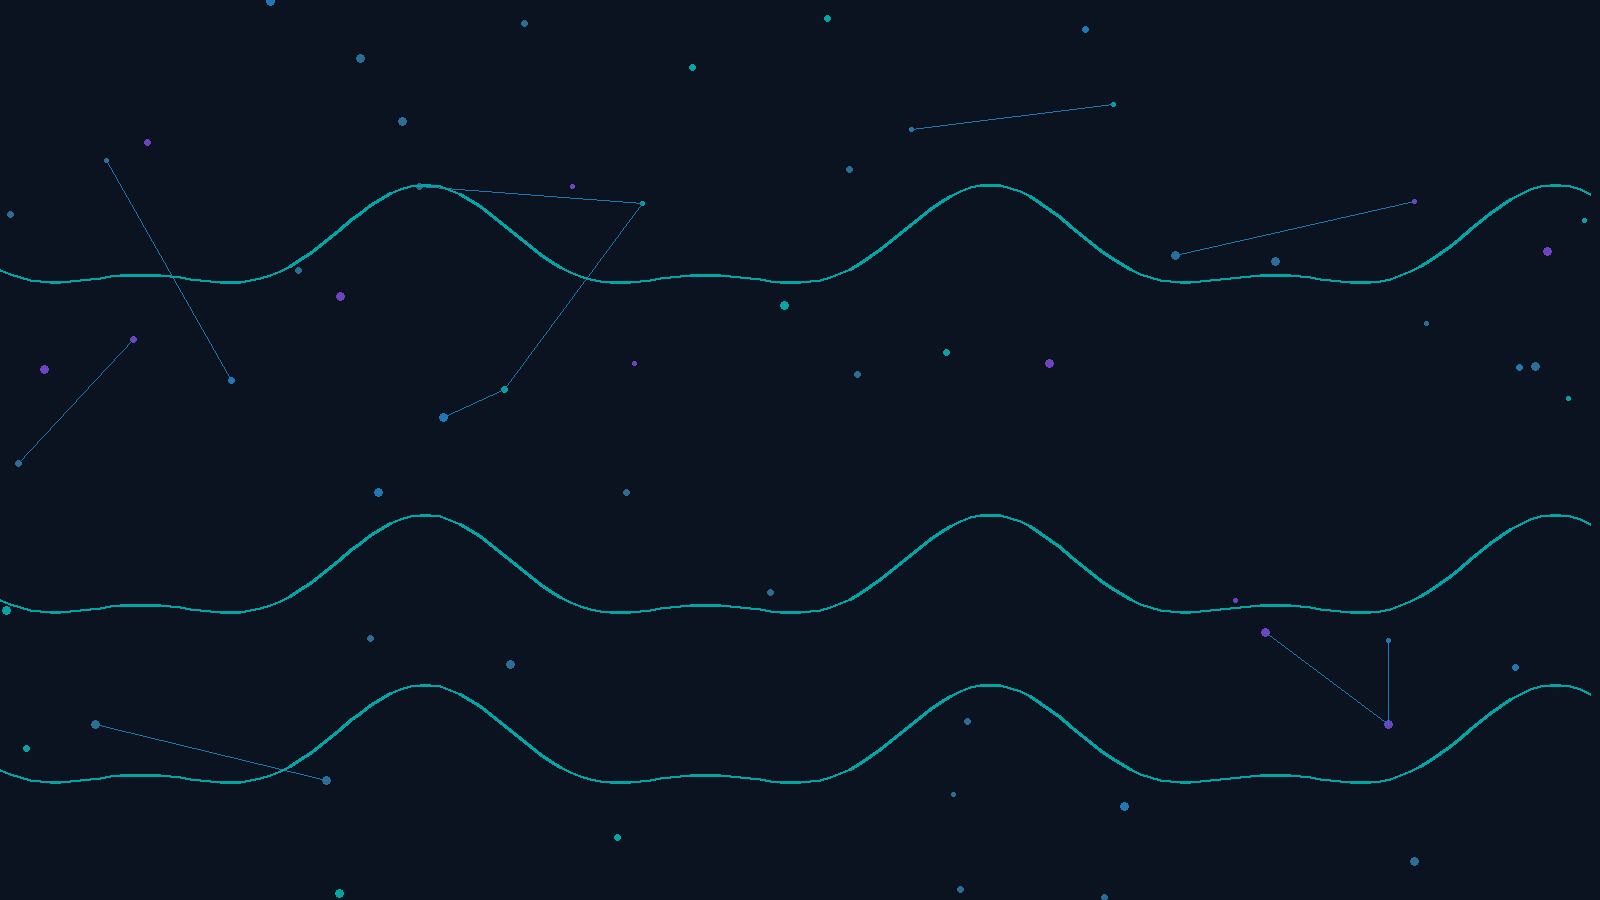
\includegraphics[width=\paperwidth,height=\paperheight]{../M05/assets/tech_bg.png}};%
}{\IfFileExists{../M01/assets/tech_bg.png}{\node[anchor=center] at (current page.center){
\includegraphics[width=\paperwidth,height=\paperheight]{../M01/assets/tech_bg.png}};}{\fill[DeepNavy!7] (current page.south west) rectangle (current page.north east);}}
\fill[DeepNavy,opacity=.84] (current page.south west) rectangle ([xshift=8.15cm]current page.north west);
\node[anchor=north west,text=white,align=left,text width=7.0cm] at ([xshift=.65cm,yshift=-.55cm]current page.north west){%
{\hyphenpenalty=10000\exhyphenpenalty=10000\fontsize{20}{22.5}\selectfont\bfseries Pertemuan 10\\Klasifikasi dengan\\K-Nearest Neighbors}\\[3mm]
{\fontsize{14.5}{17}\selectfont Pemrograman untuk Ilmu Data\\dan Komputasi}\\[2.5mm]
{\fontsize{10.5}{12}\selectfont MA25-21008 \quad Kelas RA dan RB}\\[5mm]
{\fontsize{10}{11.5}\selectfont \textbf{Triyana Muliawati, S.Si., M.Si.}\\Rifky Fauzi}\\[3mm]
{\fontsize{9.3}{10.8}\selectfont Program Studi Matematika\\Institut Teknologi Sumatera\\Semester Ganjil 2026/2027}
};
\node[anchor=north east,fill=white,fill opacity=.95,text opacity=1,rounded corners=3pt,inner sep=4.0mm,text width=6.95cm] at ([xshift=-.35cm,yshift=-.78cm]current page.north east){%
{\fontsize{13}{15}\selectfont\bfseries Pokok bahasan}\\[2mm]
\begin{itemize}\small
  \item Klasifikasi sebagai masalah prediksi kategori.
  \item Representasi fitur dan label kelas.
  \item Jarak Euclidean dan konsep tetangga terdekat.
  \item Algoritma K-Nearest Neighbors (KNN).
  \item Implementasi KNN dari prinsip matematika dengan NumPy.
  \item Kompleksitas algoritma, skala fitur, dan evaluasi.
\end{itemize}
};
\end{tikzpicture}
\end{frame}

% 2
\begin{frame}{Dari Data ke Keputusan}
\begin{columns}[T]
\column{.50\textwidth}
\IfFileExists{assets/data_information_knowledge_insight_wisdom_impact.jpg}{%
\centering
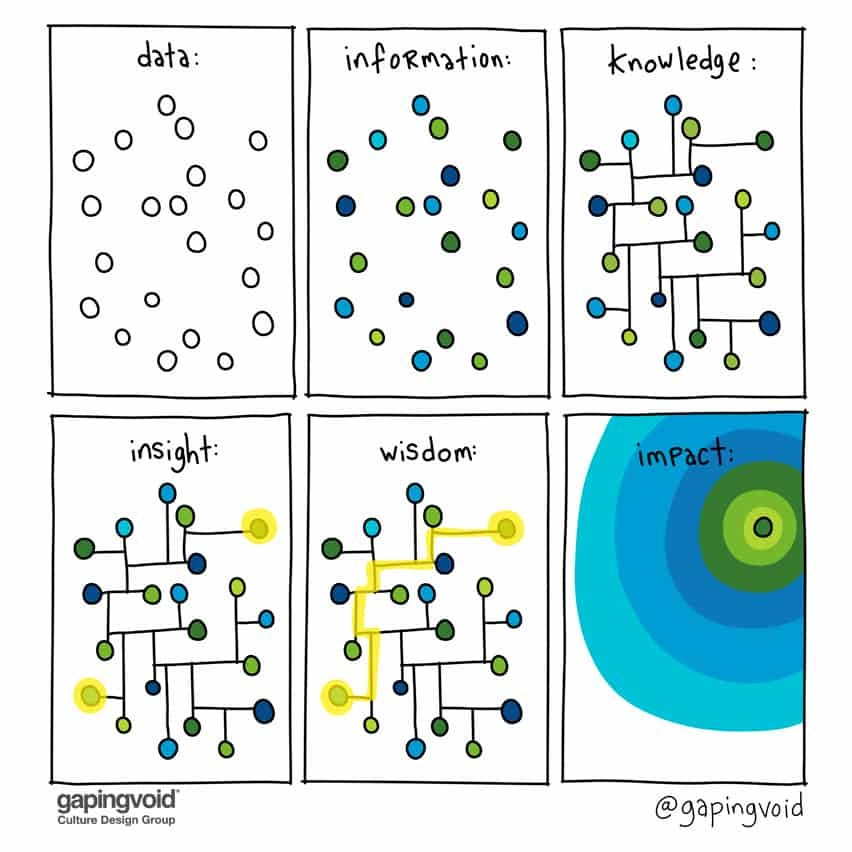
\includegraphics[height=6.55cm]{assets/data_information_knowledge_insight_wisdom_impact.jpg}
\par\vspace{.3mm}
{\tiny Ilustrasi: Gapingvoid Culture Design Group (gambar terlampir).}
}{%
\begin{block}{Ilustrasi}
Data menjadi berguna ketika kita mengenali struktur, hubungan, dan keputusan yang dapat diambil darinya.
\end{block}
}
\column{.46\textwidth}
\begin{block}{Dari titik menjadi kelas}
\footnotesize
Pada gambar, titik yang semula belum dibedakan mulai memperoleh \textbf{label} dan \textbf{hubungan}. Dalam klasifikasi, label dapat berupa warna, kategori, atau nama kelas.
\end{block}
\begin{alertblock}{Pertanyaan komputasi}
\footnotesize
Jika beberapa objek sudah diketahui kelasnya, dapatkah kita menentukan \textbf{kelas objek baru} berdasarkan objek yang sudah ada?
\end{alertblock}
\begin{block}{Hubungan dengan pertemuan sebelumnya}
\footnotesize
Regresi memprediksi \textbf{nilai numerik}; klasifikasi memprediksi \textbf{kelas/kategori}.
\end{block}
\end{columns}
\end{frame}

% 3
\begin{frame}{Klasifikasi: Apa yang Diprediksi?}
\begin{columns}[T]
\column{.49\textwidth}
\begin{block}{Regresi pada pertemuan sebelumnya}
\small
Output model berupa nilai numerik:
\[
\hat y \in \mathbb{R}.
\]
Contoh:
\begin{itemize}
  \item prediksi nilai ujian;
  \item estimasi harga rumah;
  \item perkiraan konsumsi listrik.
\end{itemize}
\end{block}
\column{.47\textwidth}
\begin{block}{Klasifikasi}
\small
Output model berupa kategori:
\[
\hat y \in \{C_1,C_2,\ldots,C_m\}.
\]
Contoh:
\begin{itemize}
  \item email: spam / bukan spam;
  \item transaksi: fraud / normal;
  \item objek: kelas A / B / C.
\end{itemize}
\end{block}
\end{columns}
\begin{alertblock}{Gagasan utama}
Klasifikasi menggunakan pola pada data berlabel untuk menentukan label data baru. Ini merupakan bentuk \textbf{supervised learning}.
\end{alertblock}
\end{frame}

% 4
\begin{frame}{Masalah Klasifikasi Dua Fitur}
\begin{columns}[T]
\column{.47\textwidth}
\begin{block}{Contoh sederhana}
\small
Misalkan setiap mahasiswa direpresentasikan oleh
\[
x=(x_1,x_2),
\]
dengan $x_1$ = persentase kehadiran dan $x_2$ = nilai tugas. Labelnya
\[
y\in\{\text{Lulus},\text{Belum}\}.
\]
Data yang sudah ada mempunyai fitur dan label. Untuk mahasiswa baru, fitur diketahui tetapi label belum diketahui.
\end{block}
\column{.49\textwidth}
\centering
\begin{tikzpicture}[x=.60cm,y=.49cm]
  \draw[->,thick] (0,0) -- (8.2,0) node[right]{\scriptsize $x_1$};
  \draw[->,thick] (0,0) -- (0,7.2) node[above]{\scriptsize $x_2$};
  \foreach \p in {(1.4,1.5),(2.0,2.0),(2.5,1.6),(2.8,2.7),(3.2,2.1)}
    \fill[Blue] \p circle (2.2pt);
  \foreach \p in {(5.0,4.8),(5.7,5.3),(6.2,4.4),(6.5,5.8),(5.4,6.1)}
    \fill[Teal!80!black] \p circle (2.2pt);
  \draw[very thick,Gold!85!black] (4.1,3.8) circle (3.2pt);
  \node[anchor=west] at (4.25,3.8){\scriptsize objek baru};
  \node[Blue] at (2.0,6.6){\scriptsize Kelas A};
  \node[Teal!80!black] at (6.1,6.6){\scriptsize Kelas B};
\end{tikzpicture}
\vspace{1mm}
\begin{alertblock}{Coba tebak sebelum menghitung}
\footnotesize
Kelas mana yang Anda pilih untuk titik kuning? Alasan paling sederhana biasanya: \textbf{lihat objek-objek yang paling dekat}.
\end{alertblock}
\end{columns}
\end{frame}

% 5
\begin{frame}{Intuisi Tetangga Terdekat}
\begin{columns}[T]
\column{.49\textwidth}
\centering
\begin{tikzpicture}[x=.68cm,y=.55cm]
  \draw[->,thick] (0,0) -- (8.0,0);
  \draw[->,thick] (0,0) -- (0,7.0);
  \foreach \p in {(1.5,1.5),(2.2,2.0),(2.8,2.8),(3.0,1.6),(3.6,2.4)}
    \fill[Blue] \p circle (2.4pt);
  \foreach \p in {(5.0,4.8),(5.5,5.5),(6.0,4.1),(6.6,5.2),(5.9,6.1)}
    \fill[Teal!80!black] \p circle (2.4pt);
  \coordinate (Q) at (4.35,3.55);
  \draw[Gold!90!black,line width=1.3pt] (Q) circle (3.4pt);
  \draw[Gold!70!black,dashed,thick] (Q) circle (1.75cm);
  \node[anchor=west] at (4.55,3.55){\scriptsize $x^*$};
\end{tikzpicture}
\column{.47\textwidth}
\begin{block}{Cara manusia menebak}
\small
Untuk titik baru $x^*$, kita melihat titik-titik yang paling dekat. Jika sebagian besar tetangga terdekat berasal dari Kelas A, kita cenderung menempatkan $x^*$ ke Kelas A.
\end{block}
\begin{alertblock}{Dari intuisi menjadi algoritma}
\small
Kita perlu menentukan:
\begin{enumerate}
  \item apa arti ``dekat'';
  \item berapa banyak tetangga yang dipakai;
  \item bagaimana memilih kelas dari tetangga tersebut.
\end{enumerate}
\end{alertblock}
\end{columns}
\end{frame}

% 6
\begin{frame}{K-Nearest Neighbors untuk Klasifikasi}
\small
Diberikan data latih
\[
D=\{(x_i,y_i)\}_{i=1}^{n},\qquad x_i\in\mathbb{R}^{d},\quad y_i\in\{C_1,\ldots,C_m\}.
\]
Untuk objek baru $x^*$, KNN menentukan kelas menggunakan $k$ objek data latih yang jaraknya paling dekat dengan $x^*$.
\begin{columns}[T]
\column{.49\textwidth}
\begin{block}{Masukan}
\begin{itemize}\small
  \item matriks fitur $X\in\mathbb{R}^{n\times d}$;
  \item label $y$ sebanyak $n$ buah;
  \item objek baru $x^*\in\mathbb{R}^{d}$;
  \item bilangan bulat $k$.
\end{itemize}
\end{block}
\column{.47\textwidth}
\begin{block}{Keluaran}
\small
Kelas dengan jumlah suara terbesar di antara $k$ tetangga terdekat:
\[
\hat y(x^*)=
\operatorname*{arg\,max}_{c}
\sum_{i\in N_k(x^*)}\mathbf{1}(y_i=c).
\]
\end{block}
\end{columns}
\begin{alertblock}{Ciri penting}
KNN tidak mencari parameter seperti $\beta_0,\beta_1$ pada regresi. Data latih disimpan dan digunakan ketika prediksi dilakukan.
\end{alertblock}
\end{frame}

% 7
\begin{frame}{Jarak Euclidean}
\begin{columns}[T]
\column{.52\textwidth}
\begin{block}{Dari Teorema Pythagoras}
Untuk dua titik dua dimensi
\[
x=(x_1,x_2),\qquad z=(z_1,z_2),
\]
jaraknya adalah
\[
d(x,z)=\sqrt{(x_1-z_1)^2+(x_2-z_2)^2}.
\]
Untuk $d$ fitur:
\[
\boxed{d(x,z)=\sqrt{\sum_{j=1}^{d}(x_j-z_j)^2}}
\]
\end{block}
\column{.44\textwidth}
\centering
\begin{tikzpicture}[x=1.05cm,y=.86cm]
  \draw[->,thick] (0,0) -- (4.7,0) node[right]{\scriptsize $x_1$};
  \draw[->,thick] (0,0) -- (0,4.5) node[above]{\scriptsize $x_2$};
  \coordinate (A) at (1.0,1.1);
  \coordinate (B) at (4.0,3.6);
  \fill[Blue] (A) circle (2.5pt) node[below left]{\scriptsize $x$};
  \fill[Teal!80!black] (B) circle (2.5pt) node[above right]{\scriptsize $z$};
  \draw[dashed] (A) -- (4.0,1.1) -- (B);
  \draw[thick,Navy] (A) -- (B);
  \node at (2.65,2.55){\scriptsize $d(x,z)$};
  \node[below] at (2.5,1.1){\scriptsize $|z_1-x_1|$};
  \node[right] at (4.0,2.35){\scriptsize $|z_2-x_2|$};
\end{tikzpicture}
\begin{alertblock}{Makna}
Semakin kecil jarak, semakin mirip posisi dua objek dalam ruang fitur.
\end{alertblock}
\end{columns}
\end{frame}

% 8
\begin{frame}{Algoritma KNN untuk Klasifikasi}
\begin{block}{Input}
\small Data latih $(X,y)$, objek baru $x^*$, dan jumlah tetangga $k$.
\end{block}
\begin{enumerate}\small
  \item Hitung jarak $d_i=d(x_i,x^*)$ untuk setiap data latih $i=1,\ldots,n$.
  \item Urutkan data berdasarkan $d_i$ dari yang terkecil.
  \item Ambil indeks $k$ data pertama: $N_k(x^*)$.
  \item Ambil label dari $k$ tetangga tersebut.
  \item Hitung banyak kemunculan setiap label.
  \item Pilih label dengan frekuensi terbesar sebagai $\hat y(x^*)$.
\end{enumerate}
\begin{alertblock}{Yang perlu dapat ditelusuri}
Mahasiswa harus dapat menjelaskan: jarak mana yang dihitung, urutan tetangga, $k$ indeks terpilih, jumlah suara tiap kelas, dan keputusan akhir.
\end{alertblock}
\end{frame}

% 9
\begin{frame}{Contoh Perhitungan Manual}
\small
Gunakan dua kelas, A dan B, dengan objek baru $x^*=(3.1,2.7)$ dan $k=3$.
\begin{columns}[T]
\column{.56\textwidth}
\centering
\begin{tabular}{c c c c}
\toprule
Objek & Titik & Kelas & $d(x_i,x^*)$ \\
\midrule
1 & $(1,1)$ & A & $2.70$ \\
2 & $(2,1)$ & A & $2.03$ \\
3 & $(2,2)$ & A & $1.30$ \\
4 & $(4,4)$ & B & $1.58$ \\
5 & $(5,4)$ & B & $2.30$ \\
6 & $(4,5)$ & B & $2.47$ \\
\bottomrule
\end{tabular}
\vspace{2mm}
\begin{block}{Tiga jarak terkecil}
\small
Objek 3 (A), objek 4 (B), objek 2 (A).
\end{block}
\column{.40\textwidth}
\begin{block}{Voting}
\[
\text{A}:2\text{ suara},\qquad
\text{B}:1\text{ suara}.
\]
Maka
\[
\boxed{\hat y(x^*)=\text{A}}
\]
\end{block}
\begin{alertblock}{Perhatikan}
KNN tidak ``membuat garis'' terlebih dahulu. Keputusan ditentukan dari posisi $x^*$ terhadap data yang sudah berlabel.
\end{alertblock}
\end{columns}
\end{frame}

% 10
\begin{frame}{Pengaruh Nilai $k$}
\begin{columns}[T]
\column{.31\textwidth}
\begin{block}{$k=1$}
\small
Keputusan hanya mengikuti satu tetangga terdekat.
\begin{itemize}
  \item sangat lokal;
  \item sensitif terhadap noise atau data pencilan.
\end{itemize}
\end{block}
\column{.31\textwidth}
\begin{block}{$k$ sedang}
\small
Beberapa tetangga ikut memberikan suara.
\begin{itemize}
  \item keputusan lebih stabil;
  \item pola lokal masih dipertahankan.
\end{itemize}
\end{block}
\column{.31\textwidth}
\begin{block}{$k$ terlalu besar}
\small
Banyak data yang jauh ikut memengaruhi keputusan.
\begin{itemize}
  \item pola lokal dapat hilang;
  \item kelas mayoritas global dapat mendominasi.
\end{itemize}
\end{block}
\end{columns}
\vspace{2mm}
\begin{alertblock}{Catatan praktis}
Untuk dua kelas, $k$ ganjil sering dipilih untuk mengurangi peluang hasil voting seri. Nilai $k$ tetap perlu dievaluasi pada data yang tidak digunakan sebagai tetangga ``jawaban'' saat pemilihan model.
\end{alertblock}
\end{frame}

% 11
\begin{frame}[fragile]{Implementasi KNN dari Prinsip Matematika}
\begin{columns}[T]
\column{.56\textwidth}
\begin{lstlisting}
import numpy as np

def knn_predict(X, y, x_new, k=3):
    # 1. jarak Euclidean ke semua data
    diff = X - x_new
    jarak = np.sqrt(np.sum(diff**2, axis=1))

    # 2. urutkan jarak, ambil k terdekat
    idx = np.argsort(jarak)[:k]
    label_tetangga = y[idx]

    # 3. voting mayoritas
    label, jumlah = np.unique(
        label_tetangga,
        return_counts=True
    )
    prediksi = label[np.argmax(jumlah)]

    return prediksi, jarak, idx
\end{lstlisting}
\column{.40\textwidth}
\begin{block}{Yang terjadi di dalam kode}
\small
\begin{enumerate}
  \item pengurangan vektor fitur;
  \item kuadrat dan penjumlahan;
  \item akar kuadrat;
  \item sorting indeks;
  \item penghitungan frekuensi label.
\end{enumerate}
\end{block}
\begin{alertblock}{Bukan black box}
Kita belum memakai pustaka pemodelan. NumPy hanya membantu menjalankan operasi matematis dan algoritmik yang sudah dipahami.
\end{alertblock}
\end{columns}
\end{frame}

% 12
\begin{frame}[fragile]{Tracing Implementasi KNN}
\begin{columns}[T]
\column{.52\textwidth}
\begin{lstlisting}
X = np.array([
    [1, 1], [2, 1], [2, 2],
    [4, 4], [5, 4], [4, 5]
], dtype=float)

y = np.array(["A", "A", "A",
              "B", "B", "B"])

x_new = np.array([3.1, 2.7])

pred, jarak, idx = knn_predict(
    X, y, x_new, k=3
)

print(jarak)
print(idx)
print(y[idx])
print(pred)
\end{lstlisting}
\column{.44\textwidth}
\begin{block}{Hasil yang harus dapat dijelaskan}
\small
\begin{itemize}
  \item `jarak`: satu nilai untuk setiap baris $X$;
  \item `idx`: indeks tiga jarak terkecil;
  \item `y[idx]`: label para tetangga;
  \item `pred`: hasil voting mayoritas.
\end{itemize}
\end{block}
\begin{alertblock}{Pertanyaan code defense}
Jika $k$ diubah dari 3 menjadi 5, bagian mana dari algoritma yang berubah dan bagian mana yang tetap sama?
\end{alertblock}
\end{columns}
\end{frame}

% 13
\begin{frame}{Kompleksitas Algoritma KNN}
\small
Misalkan terdapat $n$ data latih dan $d$ fitur. Untuk implementasi sederhana yang memakai \texttt{argsort}:
\begin{columns}[T]
\column{.54\textwidth}
\centering
\begin{tabular}{l l c}
\toprule
Langkah & Operasi & Big-O \\
\midrule
Hitung jarak & $n\times d$ komponen & $O(nd)$ \\
Urutkan jarak & sorting $n$ nilai & $O(n\log n)$ \\
Ambil tetangga & $k$ indeks & $O(k)$ \\
Voting & $k$ label & $O(k)$ \\
\bottomrule
\end{tabular}
\column{.42\textwidth}
\begin{block}{Total prediksi sederhana}
\[
T(n,d,k)=O(nd+n\log n+k).
\]
Jika $d$ dianggap tetap:
\[
T(n)=O(n\log n).
\]
\end{block}
\begin{alertblock}{Konsekuensi}
KNN sederhana pada tahap ``belajar'', tetapi prediksi tetap perlu menghitung jarak terhadap data latih.
\end{alertblock}
\end{columns}
\end{frame}

% 14
\begin{frame}{Skala Fitur Memengaruhi Jarak}
\begin{columns}[T]
\column{.49\textwidth}
\begin{block}{Masalah}
\small
Misalkan dua fitur adalah:
\begin{itemize}
  \item usia: sekitar $18$--$60$;
  \item pendapatan: sekitar $2{,}000{,}000$--$20{,}000{,}000$.
\end{itemize}
Pada jarak Euclidean, fitur dengan skala sangat besar dapat mendominasi hasil jarak.
\end{block}
\column{.47\textwidth}
\begin{block}{Standardisasi}
\small
Salah satu pendekatan adalah mengubah fitur menjadi
\[
z_{ij}=\frac{x_{ij}-\mu_j}{s_j},
\]
dengan $\mu_j$ rata-rata dan $s_j$ simpangan baku fitur ke-$j$ pada data latih.
\end{block}
\begin{alertblock}{Prinsip penting}
Parameter skala dihitung dari \textbf{data latih}, lalu digunakan kembali untuk mentransformasi data uji atau objek baru.
\end{alertblock}
\end{columns}
\end{frame}

% 15
\begin{frame}{Evaluasi Hasil Klasifikasi}
\begin{columns}[T]
\column{.49\textwidth}
\begin{block}{Data latih dan data uji}
\small
Data latih dipakai sebagai tetangga berlabel. Data uji digunakan untuk memeriksa apakah aturan KNN juga bekerja pada objek yang tidak dipakai sebagai acuan keputusan.
\end{block}
\begin{block}{Akurasi}
\[
\text{akurasi}
=\frac{\text{jumlah prediksi benar}}
{\text{jumlah data uji}}.
\]
\end{block}
\column{.47\textwidth}
\begin{block}{Matriks kebingungan dua kelas}
\centering
\begin{tabular}{c|cc}
 & Pred. A & Pred. B \\
\hline
Aktual A & benar A & salah ke B \\
Aktual B & salah ke A & benar B
\end{tabular}
\end{block}
\begin{alertblock}{Bukan hanya nilai akurasi}
Periksa juga jenis kesalahan: kelas mana yang sering tertukar dan apakah jumlah anggota tiap kelas seimbang.
\end{alertblock}
\end{columns}
\end{frame}

% 16
\begin{frame}{Latihan: KNN dari Perhitungan hingga Algoritma}
\scriptsize
\begin{columns}[T]
\column{.48\textwidth}
Gunakan data berikut.
\vspace{1mm}
\centering
\begin{tabular}{c c c c}
\toprule
No & $x_1$ & $x_2$ & Kelas \\
\midrule
1 & 1 & 1 & A \\
2 & 2 & 1 & A \\
3 & 2 & 2 & A \\
4 & 3 & 2 & A \\
5 & 3 & 3 & A \\
6 & 5 & 4 & B \\
7 & 5 & 5 & B \\
8 & 6 & 4 & B \\
9 & 6 & 5 & B \\
10 & 7 & 5 & B \\
\bottomrule
\end{tabular}
\column{.48\textwidth}
\begin{block}{Tugas}
\begin{enumerate}
  \item Untuk $x^*=(4.2,3.2)$, hitung seluruh jarak Euclidean.
  \item Urutkan jarak dan tentukan prediksi untuk $k=3$.
  \item Ulangi untuk $k=5$. Apakah hasilnya berubah?
  \item Implementasikan fungsi KNN menggunakan NumPy tanpa pustaka pemodelan.
  \item Tampilkan indeks tetangga dan labelnya sebagai bagian tracing.
  \item Tuliskan $T(n,d,k)$ dan Big-O algoritma yang digunakan.
\end{enumerate}
\end{block}
\begin{alertblock}{Tujuan}
Bukan sekadar memperoleh kelas akhir, tetapi dapat menjelaskan hubungan antara rumus jarak, sorting, voting, kode, dan kompleksitas algoritma.
\end{alertblock}
\end{columns}
\end{frame}

% 17
\begin{frame}{Ringkasan}
\begin{columns}[T]
\column{.49\textwidth}
\begin{block}{Klasifikasi}
\small
Memetakan objek dengan fitur $x$ ke salah satu kelas yang tersedia.
\end{block}
\begin{block}{KNN}
\small
Keputusan didasarkan pada $k$ data berlabel yang paling dekat menurut suatu ukuran jarak.
\end{block}
\column{.47\textwidth}
\begin{block}{Komponen matematis}
\small
Ruang fitur, jarak Euclidean, urutan jarak, dan voting mayoritas.
\end{block}
\begin{block}{Komponen algoritmik}
\small
Perulangan/operasi vektor untuk jarak, sorting, pemilihan $k$ indeks, counting label, serta analisis kompleksitas.
\end{block}
\end{columns}
\begin{alertblock}{Inti pembelajaran}
KNN menunjukkan bahwa sebuah metode machine learning dapat dipahami sebagai rangkaian operasi matematika dan algoritma yang sederhana, transparan, dan dapat ditelusuri.
\end{alertblock}
\vspace{1mm}
{\tiny Bacaan: James et al., \textit{An Introduction to Statistical Learning}, 2nd ed.; Hastie, Tibshirani, Friedman, \textit{The Elements of Statistical Learning}, 2nd ed.}
\end{frame}

\end{document}

